\section{Accelerated Methods}

The intuition behind using accelerated methods is that it introduces a
physics-inspired component to GD which mimics a dampened oscillator ordinary
differential equation (ODE). This effect minimizes the oscillations that tend to
occur in gradient descent by using previous gradient computations to penalize
rapid changes in direction and reward movement towards an optimal point.

\subsection{Polyak's Momentum}%
\label{sub:polyak_s_momentum}

We reconstruct this via a method similar to as was done by
\citeauthor{10.1214/18-EJS1395}: the ODE limit for gradient descent is given by
the equation
\begin{equation}
    \dv{x}{t} = -\nabla f(x).
\end{equation}
This can be modified to mimic a dampened oscillator ODE by including acceleration
and dampening term $\gamma \geq 0$
\begin{equation}
    \dv{^2 x}{t^2}  + \gamma \dv{x}{t} = -\nabla f(x)
\end{equation}
and then rearranged to interpret in terms of acceleration, along with a
simplification to velocity $v$ of $x$, i.e.  $v = \dv{x}{t}$,
\begin{equation}
    \dv{v}{t}  =  -\gamma v -\nabla f(x).
\end{equation}
Conversion to a discrete time step $\sqrt{\eta}$ with a forward-difference yields the equations
\begin{equation}
    \label{eq:der}
    \dv{v_t}{t} \approx \frac{v_{t + 1} - v_t}{\sqrt{\eta}}, \quad \text{and}
    \quad v_{t} = \dv{x_t}{t} \approx \frac{x_{t + 1} - x_t}{\sqrt{\eta}}
\end{equation}
which can be used to derive a formula for the dampened oscillator GD. Let $\beta
= 1 - \gamma \sqrt{\eta}$. Then at iteration $t - 1$
\begin{equation}
    \label{eq:formula}
    \begin{aligned}
        \frac{v_{t} - v_{t - 1}}{\sqrt{\eta}} &= -\gamma v_{t - 1} -\nabla
        f(x_{t - 1}) \\
        v_{t} - v_{t - 1} &= -\gamma\sqrt\eta v_{t - 1} -\sqrt \eta \nabla
        f(x_{t - 1}) \\
        v_{t} &= \beta v_{t - 1} - \sqrt{\eta} \nabla f(x_{t - 1})\\
        \frac{x_{t + 1} - x_t}{\sqrt{\eta}} &= \beta \frac{x_{t}
        - x_{t - 1}}{\sqrt{\eta}} - \sqrt{\eta} \nabla f(x_{t - 1}) \\
        x_{t + 1} &= x_t + \beta (x_{t} - x_{t - 1}) - \eta \nabla f(x_{t - 1})
    \end{aligned}
\end{equation}
By modifying this equation to evaluate the gradient at $x_t$ rather
than $x_{t - 1}$, this yields the \emph{heavyball} method as was discovered by
\citeauthor{heavyball}
\begin{equation}
    \label{eq:heavyball}
        x_{t + 1} = x_t + \beta (x_{t} - x_{t - 1}) - \eta \nabla f(x_t).
\end{equation}


\subsection{Nesterov's Momentum}%
\label{sub:nesterov_s_momentum}




Despite the effectiveness of this method, Polyak's still has the potential to
oscillate infinitely under specific conditions, as observed by
\citeauthor{lessard2016analysis}. This is due to the gradient being evaluated
\emph{before} momentum is applied and $x_t$ sometimes serving as a poor approximate
for $x_{t - 1}$. \citeauthor{nesterov1983method} altered this method slightly by
evaluating the gradient \emph{after} momentum is applied.  This derivation can
be made by reinterpreting Equation~\ref{eq:der} as a backwards difference with time
step $\sqrt\delta$ for some $\delta \geq 0$
\begin{equation}
    \label{eq:der}
    \dv{v_t}{t} \rightarrow \frac{v_{t} - v_{t - 1}}{\sqrt{\delta}}, \quad \text{and}
    \quad v_{t} = \dv{x_t}{t} \rightarrow \frac{x_{t} - x_{t - 1}}{\sqrt{\delta}}
\end{equation}
and re-deriving Equation~\ref{eq:formula} under this condition. Let $\beta =
{\left( 1 + \gamma \sqrt{\delta} \right) }^{-1}$ and $\eta = \beta \delta$. Then
at iteration $t + 1$
\begin{equation}
    \label{eq:formula}
    \begin{aligned}
        \frac{v_{t + 1} - v_{t}}{\sqrt{\delta}} &= -\gamma v_{t + 1} -\nabla
        f(x_{t + 1}) \\
        v_{t + 1} - v_{t} &= -\gamma \sqrt{\delta}v_{t + 1} -\sqrt{\delta}\nabla
        f(x_{t + 1}) \\
        \beta^{-1}v_{t + 1} - v_{t} &= -\sqrt{\delta}\nabla
        f(x_{t + 1}) \\
        \frac{x_{t + 1} - x_{t}}{\beta\sqrt{\delta}} - \frac{x_{t} - x_{t - 1}}{\sqrt{\delta}} &=  -\sqrt{\delta}\nabla
        f(x_{t + 1}) \\
        \frac{x_{t + 1} - x_{t}}{\beta\sqrt{\delta}} &= \frac{x_{t} - x_{t -
        1}}{\sqrt{\delta}} - \sqrt{\delta}\nabla f(x_{t + 1}) \\
        x_{t + 1} - x_{t} &= \beta (x_{t} - x_{t -
        1}) - \eta \nabla f(x_{t + 1}) \\
        x_{t + 1} &= x_{t} + \beta (x_{t} - x_{t -
        1}) - \eta \nabla f(x_{t + 1}).
    \end{aligned}
\end{equation}

By evaluating the gradient at $x_t + \beta(x_t - x_{t - 1})$ rather than $x_{t +
1}$, this then yields Nesterov's accelerated method.
\begin{equation}
    x_{t + 1} = x_t + \beta (x_t - x_{t - 1}) - \eta \nabla f(x_t + \beta (x_t - x_{t -
    1})).
\end{equation}
The difference between these methods is shown in
Figure~\ref{fig:sc1-png}.

\begin{research}
    Heavyball and Nesterov's momentum use either forward or backwards
    differences, which both yield a $\mathcal O(\epsilon)$ derivative approximation.
    Center differences, defined at time step $t$ by 
    \begin{equation}
        \dv{x_t}{t} \approx \frac{x_{t + 1} - x_{t - 1}}{\delta} 
    \end{equation}
    have been shown to yield a $\mathcal O(\epsilon^2)$ approximation [citation
    needed]. Would there be any performance benefits to using this derivative
    approximation over the other momentum methods?
\end{research}

\begin{figure}[t]
    \centering
    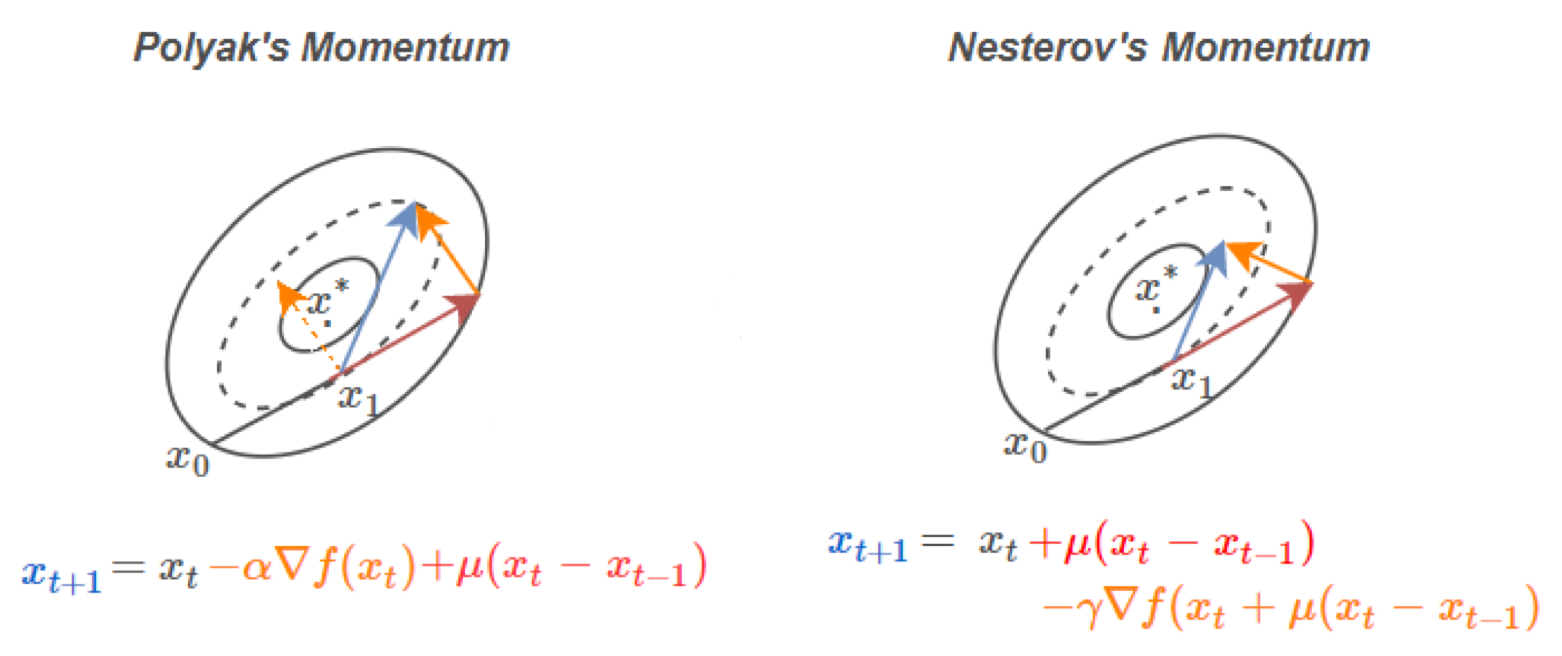
\includegraphics[width=0.8\textwidth]{sc1.png}
    \caption{Comparison between
    Polyak’s and Nesterov’s momentum. The gradient descent step (orange arrow)
    is perpendicular to the level set before applying momentum to $x_1$ (red
    arrow) in Polyak’s algorithm, whereas it is perpendicular to the level set
    after applying momentum to $x_1$ in Nesterov’s algorithm. Graphic provided by \citeauthor{nesterovnotes}.}
    \label{fig:sc1-png}
\end{figure}
